\chapter{Minimizing Logic Functions}
\label{ch:minimize}

% Helper commands for four-variable Karnaugh maps.
% \kmapfour{16 values in map row order: 0, 1 or x} draws the labels and cells
% (rows AB = 00,01,11,10; columns CD = 00,01,11,10); the corner of each cell shows the minterm number.
% \kgrp{colour}{column1}{row1}{column2}{row2}{margin} outlines a rectangular group.
\providecommand{\kmapfour}[1]{%
  \foreach \kc/\klab in {0/00, 1/01, 2/11, 3/10} \node[font=\sffamily\small] at (\kc,0.85) {\klab};
  \foreach \kr/\klab in {0/00, 1/01, 2/11, 3/10} \node[font=\sffamily\small] at (-0.95,-\kr) {\klab};
  \node[font=\sffamily\small] at (-1.2,0.85) {$AB\backslash CD$};
  \foreach \kv [count=\ki from 0] in {#1} {%
    \pgfmathtruncatemacro{\kr}{int(\ki/4)}%
    \pgfmathtruncatemacro{\kc}{mod(\ki,4)}%
    \def\kfill{white}%
    \if 1\kv \def\kfill{FpgaLight}\fi
    \if x\kv \def\kfill{gray!25}\fi
    \node[draw, minimum size=10mm, font=\sffamily\large, fill=\kfill] at (\kc,-\kr) {\if x\kv$\times$\else\kv\fi};
    \node[font=\sffamily\footnotesize, text=gray, anchor=south east, inner sep=1pt] at (\kc+0.48,-\kr-0.48) {\ifcase\ki\relax 0\or 1\or 3\or 2\or 4\or 5\or 7\or 6\or 12\or 13\or 15\or 14\or 8\or 9\or 11\else 10\fi};
  }}
\providecommand{\kgrp}[6]{\draw[very thick, #1, rounded corners=4pt]
  (#2-#6,-#3+#6) rectangle (#4+#6,-#5-#6);}

In Chapter~\ref{ch:comb} we built circuits from a truth table and simplified
them with a three-variable Karnaugh map. Some questions are still open. What
do you do when there are four variables and the map no longer fits ``on one
line''? How do you avoid mistakes when choosing groups, if the group you need
is not the largest one? What do you do with input combinations that simply
never occur? And most important: what will your ``minimal'' form turn into in
a real circuit? Here we go through the full set of techniques, while the formal
Quine algorithm and multilevel circuits are moved to the advanced sections at
the end of the chapter: you can skip them on a first reading.

\begin{buildbox}
The \emph{Learn} tab, the ``Comparison and codes'' book, the lesson
\emph{``A number in the range 3\ldots 9''}: build a circuit in which $y=1$ if
the four-bit number $x$ lies in the range from 3 to 9. Pass the automatic
check and write down how many blocks you used. At the end of the chapter we
will write the same function as $F=\Sigma m(3,4,5,6,7,8,9)$ with the
don't-care states $10$--$15$ and see whether comparators are needed at all.
\end{buildbox}

\section{Canonical Forms}

Any function can be written ``head-on'', directly from the truth table.

\begin{itemize}
  \item \term{Canonical sum of products} (SOP, or disjunctive normal form):
        for each row where $F=1$, write the product of all variables (with
        a bar over those that equal zero), and add these products together.
        Each such product is a \term{minterm} $m_i$.
  \item \term{Canonical product of sums} (POS, or conjunctive normal form):
        for each row where $F=0$, write the sum of all variables (with a bar
        over those that equal \emph{one}), and multiply these sums together.
        Each such sum is a \term{maxterm} $M_i$.
\end{itemize}

These forms are always correct, but redundant: for a function of four
variables the canonical SOP can consist of eight terms with four literals
each. The task of minimization is to find an expression with the smallest
number of terms and literals. A function is often specified by a list of row
numbers: the notation $F=\Sigma m(0,1,2,5)$ means ``the function equals one on
rows 0, 1, 2 and 5, and zero on all the others''. The row number is the value
of the inputs read as a binary number ($ABCD=0101$ is row 5).

\textbf{Example.} For $F=\Sigma m(1,6)$ of three variables $A,B,C$ the
canonical SOP is $F=\overline{A}\,\overline{B}C + AB\overline{C}$ (row 1 is
$001$, row 6 is $110$). The canonical POS for the same function would need
one factor for each of the six rows with a zero, that is, six sums. So you
should write the form in which fewer rows are ``selected'': few ones---use
the SOP, few zeros---use the POS.

How many functions are there in total? $n$ variables give $2^n$ rows, and in
each of them you can put 0 or 1, so there are $2^{2^n}$ functions: sixteen for
two variables, 256 for three, 65\,536 for four. Going through all of them by
hand is impossible, and that is exactly why systematic techniques are needed.

\begin{diybox}[Write it out and build it head-on]
\textbf{Task.} \stars{1} Write the canonical SOP of the function
$F=\Sigma m(1,6)$ and the canonical POS of the function ``$A\cdot B$ of two
variables''. \stars{2} For the function ``a number from 3 to 9'' write out the
minterms (seven of them) and count how many elements the ``head-on'' circuit
would have (inverters, AND gates with four inputs, one OR gate with seven
inputs). \stars{3} Compare this estimate with what you built at the beginning
of the chapter.

\textbf{In Logra.} The \emph{Designer} tab: a circuit of NOT, AND and OR
blocks for the function $\Sigma m(1,6)$ (three inputs).

\textbf{Expected result.} A circuit of two three-input AND gates and one
two-input OR gate plus inverters. The estimate for $3\ldots 9$ gives about
twelve elements (seven AND, four NOT, one seven-input OR)---and this is
a clear reason to simplify.

\textbf{How to check.} The \emph{Waveforms} tab: go through all the rows; the
one must appear in rows 1 and 6 only.
\end{diybox}

\section{The Four-Variable Karnaugh Map}

For four variables $A,B,C,D$ the map consists of 16 cells arranged as a
$4\times 4$ square. The rows are labelled with the values of $AB$, the columns
with $CD$, both in Gray code order: \code{00, 01, 11, 10}. Because of this,
cells that are neighbours horizontally and vertically differ in one variable.
An important consequence: \emph{the map wraps around}. The left column is
adjacent to the right one, the top row to the bottom one, and the four
corners together form one group. It is as if the map were drawn on the
surface of a doughnut.

Let us minimize the function $F = \Sigma m(0,1,2,5,8,9,10)$.

\begin{figure}[H]
\centering
\begin{tikzpicture}[cell/.style={draw, minimum size=10mm, font=\sffamily\large}]
  % labels
  \foreach \c/\lab in {0/00, 1/01, 2/11, 3/10} \node[font=\sffamily\small] at (\c,0.85) {\lab};
  \foreach \r/\lab in {0/00, 1/01, 2/11, 3/10} \node[font=\sffamily\small] at (-0.95,-\r) {\lab};
  \node[font=\sffamily\small] at (-1.2,0.85) {$AB\backslash CD$};
  % values of F
  \foreach \r/\c/\v in {0/0/1, 0/1/1, 0/2/0, 0/3/1,
                        1/0/0, 1/1/1, 1/2/0, 1/3/0,
                        2/0/0, 2/1/0, 2/2/0, 2/3/0,
                        3/0/1, 3/1/1, 3/2/0, 3/3/1}
    {\ifnum\v=1 \def\cc{FpgaLight}\else\def\cc{white}\fi
     \node[cell, fill=\cc] at (\c,-\r) {\v};}
  % group B'D': four corners
  \foreach \x/\y in {0/0, 3/0, 0/-3, 3/-3}
    \draw[very thick, FpgaRed, rounded corners=4pt] (\x-0.44,\y+0.44) rectangle (\x+0.44,\y-0.44);
  % group B'C': 2 cells at the top and 2 at the bottom (vertical wrap-around)
  \draw[very thick, FpgaGreen, rounded corners=4pt] (-0.40,0.40) rectangle (1.40,-0.40);
  \draw[very thick, FpgaGreen, rounded corners=4pt] (-0.40,-2.60) rectangle (1.40,-3.40);
  % group A'C'D: two vertical neighbours
  \draw[very thick, FpgaOrange, rounded corners=4pt] (0.68,0.30) rectangle (1.32,-1.30);
  % explanations
  \node[font=\sffamily\small, text=FpgaRed, anchor=west] at (4.4,0.5) {$\overline{B}\,\overline{D}$---four corners};
  \node[font=\sffamily\small, text=FpgaGreen, anchor=west] at (4.4,-0.3) {$\overline{B}\,\overline{C}$---top and bottom, two columns};
  \node[font=\sffamily\small, text=FpgaOrange, anchor=west] at (4.4,-1.1) {$\overline{A}\,\overline{C}\,D$---cells 1 and 5};
  \node[font=\sffamily\small\bfseries, anchor=west] at (4.4,-2.1) {$F=\overline{B}\,\overline{D}+\overline{B}\,\overline{C}+\overline{A}\,\overline{C}D$};
\end{tikzpicture}
\caption{A four-variable Karnaugh map. The red group (four corners) and the green group (two cells at the top and two at the bottom) are formed by wrapping around the edges of the map}
\label{fig:karnaugh4}
\end{figure}

The procedure is the same as for three variables:

\begin{enumerate}
  \item Mark the ones.
  \item Combine them into rectangular groups of $1, 2, 4, 8$ or 16 cells;
        groups may overlap and ``wrap around'' the edge.
  \item Take groups as large as possible and cover all the ones with the
        smallest number of groups.
  \item Each group corresponds to a product of only those variables that do
        not change within the group. A group of $2^k$ cells eliminates $k$
        variables.
\end{enumerate}

The original canonical SOP consisted of seven terms with four literals each
(28 literals), while the result has three terms with 2--3 literals each
(7 literals).

The size of a group directly determines the length of the term:

\begin{table}[H]
\centering
\caption{Group size and the number of literals in a term (4 variables)}
\begin{tabular}{c|ccccc}
\toprule
Cells in the group & 1 & 2 & 4 & 8 & 16 \\
Literals in the term & 4 & 3 & 2 & 1 & 0 (function $\equiv 1$) \\
\bottomrule
\end{tabular}
\end{table}

\subsection{Two More Examples}

\textbf{Groups of different shapes.} For $F=\Sigma m(4,5,6,7,12,13)$ the ones
form an ``L shape'': the entire row $AB=01$ (four cells) and two cells of the
row $AB=11$ beneath it.

\begin{figure}[H]
\centering
\begin{tikzpicture}
  \kmapfour{0,0,0,0, 1,1,1,1, 1,1,0,0, 0,0,0,0}
  \kgrp{FpgaRed}{0}{1}{3}{1}{0.40}
  \kgrp{FpgaGreen}{0}{1}{1}{2}{0.31}
  \node[font=\sffamily\small, text=FpgaRed, anchor=west] at (4.4,0.2) {$\overline{A}B$---the whole row $AB=01$};
  \node[font=\sffamily\small, text=FpgaGreen, anchor=west] at (4.4,-0.6) {$B\overline{C}$---the $2\times 2$ block on the left};
  \node[font=\sffamily\small\bfseries, anchor=west] at (4.4,-1.6) {$F=\overline{A}B+B\overline{C}$};
\end{tikzpicture}
\caption{Two overlapping groups: a row of four cells and a $2\times 2$ square share cells 4 and 5}
\label{fig:karnaugh4_corner}
\end{figure}

Cells $4$ and $5$ belong to both groups, and that is fine: every one must be
covered at least once, but it may be covered twice. In the row $AB=01$ the
variables $C$ and $D$ change, leaving $\overline{A}B$; in the square $A$ and
$D$ change, leaving $B\overline{C}$. In total, 4 literals instead of
$6\cdot4=24$.

\textbf{When the map does not help.} For the function ``an odd number of
ones at the input'' $F=\Sigma m(1,2,4,7,8,11,13,14)$ the ones sit in a
``checkerboard pattern'': none of them has a neighbour. All groups consist of
one cell, and the minimal form is eight terms with four literals each, that
is, the same canonical SOP. For such functions (parity, sum modulo 2) an XOR
gate is better than AND-OR: $F=A\oplus B\oplus C\oplus D$ is three two-input
XOR gates. The conclusion: before minimizing, it is useful to first look at
the map and see whether it has any large groups.

\subsection{Incorrect Grouping}

The most common beginner's mistake is to take the biggest groups first and
consider the job done. Consider $F=\Sigma m(1,5,6,7,11,12,13,15)$.

\begin{figure}[H]
\centering
\begin{tikzpicture}
  \kmapfour{0,1,0,0, 0,1,1,1, 1,1,1,0, 0,0,1,0}
  \draw[very thick, dashed, FpgaRed, rounded corners=4pt] (0.6,-0.6) rectangle (2.4,-2.4);
  \kgrp{FpgaOrange}{1}{0}{1}{1}{0.35}
  \kgrp{FpgaGreen}{2}{1}{3}{1}{0.35}
  \kgrp{FpgaBlue}{0}{2}{1}{2}{0.35}
  \kgrp{FpgaGray}{2}{2}{2}{3}{0.35}
  \node[font=\sffamily\small, text=FpgaRed, anchor=west] at (4.4,0.4) {$BD$---the central square (redundant!)};
  \node[font=\sffamily\small, text=FpgaOrange, anchor=west] at (4.4,-0.4) {$\overline{A}\,\overline{C}D$---cells 1 and 5};
  \node[font=\sffamily\small, text=FpgaGreen, anchor=west] at (4.4,-1.2) {$\overline{A}BC$---cells 6 and 7};
  \node[font=\sffamily\small, text=FpgaBlue, anchor=west] at (4.4,-2.0) {$AB\overline{C}$---cells 12 and 13};
  \node[font=\sffamily\small, text=FpgaGray, anchor=west] at (4.4,-2.8) {$ACD$---cells 11 and 15};
\end{tikzpicture}
\caption{The central square $BD$ (dashed) is larger than the others, but all its cells are already covered by four ``simple'' pairs}
\label{fig:karnaugh4_wrong}
\end{figure}

The central square $BD$ (cells 5, 7, 13, 15) is very conspicuous, and a
beginner takes it first. But let us check what remains. The one in cell~1
belongs only to the pair $\overline{A}\,\overline{C}D$, the one in cell~6
only to $\overline{A}BC$, the one in cell~11 only to $ACD$, and the one in
cell~12 only to $AB\overline{C}$. These four groups are \emph{essential}, and
together they already cover all eight ones, including 5, 7, 13 and 15. The
square $BD$ adds nothing:
\[
  F=\overline{A}\,\overline{C}D+\overline{A}BC+ACD+AB\overline{C}\quad
  (\text{without the redundant }BD).
\]
If you take $BD$ and the four essential pairs, you get five terms instead of
four: the circuit is not wrong, but it is redundant. The correct order is
this: first find the ones that can be covered in only \emph{one} way, take
those groups, and only then look at what is still uncovered.

\textbf{Other incorrect groupings.} A group of three cells or of six cells is
not allowed (the size is not a power of two). Diagonal cells never form one
group. A group cannot contain a zero unless it is a don't-care state (see the
next section). If you made a mistake, you can check the solution by
substitution: write down the resulting expression and evaluate it on several
rows, especially on the zeros.

\subsection{Minimal POS: Grouping the Zeros}

If the map has fewer zeros than ones, it is more convenient to \emph{group the
zeros}: you get the minimal form of the inverse function $\overline{F}$, and
then, by De~Morgan's law, the form for $F$ as a product of sums. For the
function $F=\Sigma m(0,1,2,5,8,9,10)$ from Figure~\ref{fig:karnaugh4} there are
nine zeros ($3,4,6,7,11,12,13,14,15$). The groups of zeros are $CD$ (cells
$3,7,11,15$), $B\overline{D}$ (cells $4,6,12,14$) and $AB$ (cells
$12,13,14,15$). Hence $\overline{F}=CD+B\overline{D}+AB$, and after
inversion
\[
  F=(\overline{C}+\overline{D})(\overline{B}+D)(\overline{A}+\overline{B}).
\]
This expression is equivalent to the sum of products found earlier. Which of
them is better depends on the needs of the circuit: in the SOP the first level
is made of AND gates, in the POS it is made of OR gates.

\begin{diybox}[Minimization with four variables]
\textbf{Task.} \stars{1} Minimize $F_1=\Sigma m(0,2,8,10)$ (the four
corners) and build it. \stars{2} For $F=\Sigma m(4,5,6,7,12,13)$ find the
minimal form and make sure that all the groups are really needed.
\stars{3} Come up with a function of four variables in which one of the
largest groups is \emph{redundant}, like the square $BD$ in our example.

\textbf{In Logra.} The \emph{Designer} tab: build a circuit from your
minimal form; then the example \code{range-check} (the example library):
compare the ``range limits'' with your own map.

\textbf{Expected result.} $F_1=\overline{B}\,\overline{D}$---one AND gate with
two inverted inputs (or one NOR gate); for $\Sigma m(4,5,6,7,12,13)$ you get
$\overline{A}B+B\overline{C}$.

\textbf{How to check.} The \emph{Waveforms} tab: apply a 0--15 counter to
$ABCD$ and compare the output with the map: the ones must appear exactly
where the map has ones. For an incorrect grouping, a check \emph{on the zeros}
will reveal an extra one.
\end{diybox}

\section{Don't-Care States}

Sometimes certain input combinations never occur at all. For example, a digit
in binary-coded decimal cannot be greater than nine: the combinations
\code{1010}--\code{1111} are forbidden in BCD. What a decoder or comparator
outputs for them does not matter. Such combinations are called
\term{don't-care states} (denoted $d$ or $\times$). They can be treated either
as zeros or as ones, depending on which gives larger groups.

\begin{figure}[H]
\centering
\begin{tikzpicture}[cell/.style={draw, minimum size=10mm, font=\sffamily\large}]
  \foreach \c/\lab in {0/00, 1/01, 2/11, 3/10} \node[font=\sffamily\small] at (\c,0.85) {\lab};
  \foreach \r/\lab in {0/00, 1/01, 2/11, 3/10} \node[font=\sffamily\small] at (-0.95,-\r) {\lab};
  \node[font=\sffamily\small] at (-1.2,0.85) {$AB\backslash CD$};
  % ``digit greater than four'': ones 5..9, don't-cares 10..15
  \foreach \r/\c/\v in {0/0/0, 0/1/0, 0/2/0, 0/3/0,
                        1/0/0, 1/1/1, 1/2/1, 1/3/1,
                        2/0/x, 2/1/x, 2/2/x, 2/3/x,
                        3/0/1, 3/1/1, 3/2/x, 3/3/x}
    {\def\cc{white}
     \if 1\v \def\cc{FpgaLight}\fi
     \if x\v \def\cc{gray!25}\fi
     \node[cell, fill=\cc] at (\c,-\r) {\if x\v$\times$\else\v\fi};}
  \draw[very thick, FpgaRed, rounded corners=4pt] (-0.40,-1.60) rectangle (3.40,-3.40);
  \draw[very thick, FpgaGreen, rounded corners=4pt] (1.60,-0.60) rectangle (3.40,-2.40);
  \draw[very thick, FpgaOrange, rounded corners=4pt] (0.60,-0.62) rectangle (2.40,-2.38);
  \node[font=\sffamily\small, text=FpgaRed, anchor=west] at (4.4,-0.3) {$A$---bottom rows (8--15)};
  \node[font=\sffamily\small, text=FpgaGreen, anchor=west] at (4.4,-1.0) {$BC$---columns $CD=11,10$};
  \node[font=\sffamily\small, text=FpgaOrange, anchor=west] at (4.4,-1.7) {$BD$---columns $CD=01,11$};
  \node[font=\sffamily\small\bfseries, anchor=west] at (4.4,-2.5) {$F = A + BC + BD$};
\end{tikzpicture}
\caption{The function ``BCD digit greater than four''. The grey cells are the don't-care states $10,\ldots,15$. Thanks to them the groups are large, and the result consists of only three terms}
\label{fig:karnaugh_dc}
\end{figure}

Without don't-care states we would have to write five separate minterms, but
with them the function turns into $F = A + BC + BD$. That is why, when
designing circuits, a designer should always ask: ``are all input combinations
possible?'' If not, then on the impossible combinations the circuit may
behave in any way, and this saves gates.

The rules for working with don't-care cells: (1) they are \emph{not required}
to be covered: the ones must be covered, while a $\times$ only if it makes the
group larger; (2) each such cell is treated separately as a zero or a one,
whichever is more convenient; (3) this works \emph{only} if the input
combinations really never occur. If an ``impossible'' code does arrive at the
input, the output will be whatever it turned out to be, and that is your
responsibility.

\textbf{A second example: ``the digit is divisible by three''.} The function
equals one on the digits $0,3,6,9$, and the codes $10$--$15$ are don't-cares.
Cell~0 is isolated: all its neighbours (1, 2, 4, 8) are zero, so the term
$\overline{A}\,\overline{B}\,\overline{C}\,\overline{D}$ stays long. But
cells 3 and 6 pair up with don't-cares: 3 with 11 gives $\overline{B}CD$, 6
with 14 gives $BC\overline{D}$, and the nine together with the don't-cares
11, 13 and 15 forms the square $AD$. The result:
\[
  F=\overline{A}\,\overline{B}\,\overline{C}\,\overline{D}+\overline{B}CD+BC\overline{D}+AD.
\]
Without don't-care states each of the last three terms would be one literal
longer, and the nine would have no neighbours at all.

\textbf{Back to the range $3\ldots9$.} The ones are in rows
$3,4,5,6,7,8,9$, and $10$--$15$ are don't-cares. Rows $8$--$15$ as a whole
(the most significant bit $A=1$) are one group of eight cells, rows $4$--$7$
and $12$--$15$ (bit $B=1$) are the second, and the foursome $3,7,11,15$
($C=D=1$) is the third. We get
\[
  F=A+B+CD.
\]
The whole circuit is one three-input OR gate and one AND gate: two blocks
instead of the two comparators, two constants and the AND gate that we built
at the beginning of the chapter. Check: on the codes $0$, $1$, $2$ there is
neither $A$, nor $B$, nor the pair $CD$, and the circuit gives $0$; on the
forbidden codes $10$--$15$ it does not matter what it gives.

\begin{infobox}[Don't-care states in hardware description languages]
In Verilog (Chapter~\ref{ch:verilog}) there is a special value \code{x} for
such a ``don't care'': the branch \code{default: y = 1'bx;} lets the
optimizer program choose the suitable variant by itself, and the circuit
comes out no larger and often smaller. An example and a comparison with the
minimal form are in Section~\ref{sec:min-verilog} below.
\end{infobox}

\begin{diybox}[Digits only up to nine]
\textbf{Task.} \stars{1} For the function ``the BCD digit is even''
($\Sigma m(0,2,4,6,8)$, $10$--$15$ are don't-cares) find the minimal form and
build it. \stars{2} Find the minimal form of the function ``the digit is
greater than four'' without using don't-care states and compare it with
$A+BC+BD$. \stars{3} Come up with a function for which don't-care states
give a gain of at least two terms.

\textbf{In Logra.} The \emph{Learn} tab, the ``Displays'' book, the lesson
\emph{``Digits only up to nine''}: there the don't-care codes $10$--$15$
blank the display. Then, in the Designer, build $F=\overline{D}$ for ``even''
and check only the digits $0$--$9$.

\textbf{Expected result.} $F=\overline{D}$ (a single inverter): the
don't-care cells $10,12,14$ extend the group to 8 cells. Without them the
function ``the digit is greater than four'' has the form
$\overline{A}BD+\overline{A}BC+A\overline{B}\,\overline{C}$ (three terms,
8 literals) instead of $A+BC+BD$ (5 literals).

\textbf{How to check.} The \emph{Waveforms} tab: going through the values
$0$--$9$ gives the expected answers; for $10$--$15$ you are not interested in
the result. But make sure that you \emph{understand} which output you get
there: a don't-care state does not guarantee a zero.
\end{diybox}

\section{From the Minimal Form to a Circuit in Logra}

Now let us connect paper and screen. Take the ``2 of 3'' function with a
guard from Chapter~\ref{ch:comb}: $y=arm\cdot(ab+ac+bc)$. This is a function
of four variables. Let $A=arm$, $B=a$, $C=b$, $D=c$; then $y=1$ on the
minterms $11,13,14,15$.

\begin{figure}[H]
\centering
\begin{tikzpicture}
  \kmapfour{0,0,0,0, 0,0,0,0, 0,1,1,1, 0,0,1,0}
  \kgrp{FpgaRed}{1}{2}{2}{2}{0.30}
  \kgrp{FpgaGreen}{2}{2}{3}{2}{0.36}
  \kgrp{FpgaOrange}{2}{2}{2}{3}{0.42}
  \node[font=\sffamily\small, text=FpgaRed, anchor=west] at (4.4,0.2) {$A B D$---cells 13 and 15};
  \node[font=\sffamily\small, text=FpgaGreen, anchor=west] at (4.4,-0.6) {$A B C$---cells 14 and 15};
  \node[font=\sffamily\small, text=FpgaOrange, anchor=west] at (4.4,-1.4) {$A C D$---cells 11 and 15};
  \node[font=\sffamily\small\bfseries, anchor=west] at (4.4,-2.3) {$y=ABD+ABC+ACD$};
\end{tikzpicture}
\caption{Security Panel, stage~3: $y = arm\cdot(ab+ac+bc)$ on a Karnaugh map ($A=arm$, $B=a$, $C=b$, $D=c$). All three groups contain cell 15}
\label{fig:karnaugh4_arm}
\end{figure}

The minimal sum of products is three terms with three literals each: three
three-input AND gates and one three-input OR gate, 4 elements and 12 inputs
in total. But you can factor $arm$ out of the brackets (see the advanced
section on multilevel circuits): $y=arm\cdot(ab+ac+bc)$ is 5 elements and 11
inputs. Which circuit is ``better'' depends on what is more expensive for
you: the number of elements or the number of levels.

\begin{infobox}[What the program does with your ``minimal'' form]
\lookahead{when a circuit turns into a real board (Chapter~\ref{ch:flow}), the optimizer
program rewrites the function itself: it does not have to repeat your minimal
form, and looks for a variant that suits the resources of the chip. In such
chips the logic is stored in small value tables with four inputs (they are
called LUTs), and any function of four variables occupies exactly one such
table regardless of the number of terms. So for a board, the number of
\emph{variables} the function depends on matters more than the number of
terms.}
\end{infobox}

Still, comparing your circuit with ``someone else's'' is useful already now:
the \emph{RTL} tab in Logra shows what your project turned into
after processing.

\begin{diybox}[Security Panel: stage 3, the minimal form]
\textbf{Task.} \stars{1} Build ``2 of 3'' with a guard in two variants:
$y=arm\cdot(ab+ac+bc)$ (5 elements) and $y=arm\,ab+arm\,ac+arm\,bc$
(4 elements, but wider). \stars{2} See how they differ on the \emph{RTL} tab.
\stars{3} \emph{A stage of the ``Security Panel'' project:} add a fourth
sensor $d$ and the condition ``at least two of four'', and find the minimal
form on the map.

\textbf{In Logra.} The \emph{Learn} tab, the ``Projects'' book, the lesson
\emph{A ``2 of 3'' vote with a guard}; then the \emph{Designer} tab for the
second variant. For the comparison use the \emph{RTL} and \emph{Gowin} tabs.

\textbf{Expected result.} Both variants have the same truth table
(4 ones out of 16 rows). For ``2 of 4'' the minimal form is six terms with
two literals each: $ab+ac+ad+bc+bd+cd$.

\textbf{How to check.} The \emph{Waveforms} tab: go through the 16
combinations of $arm\,a\,b\,c$ and compare with the map. Acceptance
criterion for stage~3: both circuits produce the same table, and the minimal
form for four inputs is written in your notebook together with the number of
groups.
\end{diybox}

\section{Don't-Care States and the Minimal Form in Verilog}
\label{sec:min-verilog}

Let us take the functions we minimized on the maps and write each of them in
two ways: as a \emph{table} (\code{case}) and as a \emph{minimal form}
(\code{assign}). The reading rules are the same as in
Section~\ref{sec:comb-verilog}; the only new thing is the value \code{x}.

\textbf{``A BCD digit greater than four'' with don't-care codes.} In the
table we describe the codes $10$--$15$ with a \code{default} branch and write
\code{1'bx} in it: ``the value does not matter''.

\vfile{\codepath/b3_comb/gt4_dc.v}{code/b3\_comb/gt4\_dc.v}

\textbf{How to read it.} The first branch lists five values (separated by
commas) with a zero output, the second five with a one; everything else falls
into \code{default}, and the output \code{x} tells the synthesizer ``choose
whatever is convenient''. The minimal form from the Karnaugh map
(Figure~\ref{fig:karnaugh_dc}) looks like this:

\vfile{\codepath/b3_comb/gt4_min.v}{code/b3\_comb/gt4\_min.v}

\textbf{How to read it.} Here $A=x[3]$, $B=x[2]$, $C=x[1]$, $D=x[0]$, so
$F=A+BC+BD$ is written with \code{x[3]}, \code{x[2]\&x[1]},
\code{x[2]\&x[0]}. On the digits $0$--$9$ both forms give the same; on the
codes $10$--$15$ the simulator shows \code{x} (undefined) for \code{gt4\_dc},
while the minimal form gives a definite value. If these codes never occur in the
real circuit, it does not matter.

\textbf{The range $3\ldots9$ in three ways.} The first is as a condition:

\vfile{\codepath/b3_comb/range3to9_cmp.v}{code/b3\_comb/range3to9\_cmp.v}

\textbf{How to read it.} \code{x >= 4'd3} is a comparison with the result 0 or
1; \code{\&\&} is the logical ``and'' of two conditions. The form reads like
the original phrase, and the synthesizer itself decides how to build the two
comparisons. The second is the minimal form $F=A+B+CD$ with the Karnaugh map
from this chapter:

\vfile{\codepath/b3_comb/range3to9_min.v}{code/b3\_comb/range3to9\_min.v}

The third is a \code{case} table where the range $3\ldots9$ is listed in one
branch and the codes $10$--$15$ are given to the don't-care \code{x}:

\vfile{\codepath/b3_comb/range3to9_case.v}{code/b3\_comb/range3to9\_case.v}

\textbf{Comparison.} On the digits $0$--$9$ the three modules give the same
table. On the codes $10$--$15$ they behave differently: the comparisons give
$0$, the minimal form gives $1$, and \code{case} with \code{x} shows an undefined
value in the simulator. All three answers are acceptable if these codes are
impossible; if they are possible, the behaviour must be chosen and written
explicitly, as in \code{default: y = 1'b0;}. The testbench \code{tb\_range.v}
checks exactly this: on $0$--$9$ all forms match the reference, and on $10$--$15$
it records what each of them gives.

\vfile{\codepath/b3_comb/tb_range.v}{code/b3\_comb/tb\_range.v}

\textbf{How to run it in Logra.} The \emph{Code} tab: paste one of the
modules, \emph{Synthesize} (Ctrl+Enter). The \emph{Waveforms} tab: $x$ from a
counter $0$--$15$ and the output $y$. For a comparison, put two modules in
the project and compare their circuits on the \emph{RTL} tab: the form with
comparisons and the minimal form give different pictures for the same table.

\begin{warnbox}[Mistakes with x and case]
\begin{itemize}
  \item \textbf{Treating \code{x} as zero.} It is not a value but ``don't care'':
        in different tools and in the simulator it may show up differently.
        If a definite behaviour is needed on forbidden codes, write 0 or 1.
  \item \textbf{Forgetting \code{default}.} Without it the output is remembered
        for the unlisted inputs and a latch results; with a \code{default}
        that assigns \code{x} there is no latch.
  \item \textbf{Mixing up the bit order.} \code{x[3]} is the most significant
        ($A$), not the least: with swapped bits you get a different function.
\end{itemize}
\end{warnbox}

\begin{diybox}[Complete and change a module]
\textbf{Task.} \stars{1} \emph{Repeat.} Type \code{range3to9\_min} and go
through all 16 values of $x$ on the waveform. \stars{2} \emph{Change it.} Do
the same for the function ``the digit is divisible by three'' (ones at
$0,3,6,9$, codes $10$--$15$ are don't-care): write it with \code{case} and
\code{default: y = 1'bx;}. \stars{3} \emph{Compare.} For the range $3\ldots9$
write one more module without don't-care codes: \code{default: y = 1'b0;},
and compare the number of blocks on the \emph{RTL} tab with the \code{x} variant.

\textbf{In Logra.} The \emph{Code} tab, \emph{Synthesize}; the \emph{RTL} and
\emph{Waveforms} tabs.

\textbf{Expected result.} \stars{2} A one at $x=0,3,6,9$ and a zero at the
other digits. \stars{3} Both modules agree on $0$--$9$; on
$10$--$15$ the second one honestly gives $0$.

\textbf{How to check.} For \stars{2} compare with the minimal form
$\overline{A}\,\overline{B}\,\overline{C}\,\overline{D}+\overline{B}CD+BC\overline{D}+AD$:
it must match on the digits $0$--$9$.
\end{diybox}

\textbf{Model answer to \stars{2}.}

\begin{vcode}
// A digit divisible by three: codes 10..15 are don't-care
module div3_dc (
    input      [3:0] x,
    output reg       y
);
    always @* begin
        case (x)
            4'd0, 4'd3, 4'd6, 4'd9:                 y = 1'b1;
            4'd1, 4'd2, 4'd4, 4'd5, 4'd7, 4'd8:     y = 1'b0;
            default:                                y = 1'bx;
        endcase
    end
endmodule
\end{vcode}

\section{Advanced Sections}

The two sections below are for those who are curious how what we did by eye
can be automated, and how the cost of a circuit depends on its depth. On a
first reading you can skip them: none of the following chapters depends on
them.

\subsection{The Quine---McCluskey Method}

The Karnaugh map is convenient for four, or maybe five, variables. For ten it
becomes a torment, and for twenty it is useless. So the programs that
simplify circuits use a formal method that can be carried out on a computer:
the \term{Quine---McCluskey method}. It consists of two parts.

\textbf{Part 1. Finding the prime implicants.} Write the minterms as binary
numbers and group them by the number of ones. Merge any two numbers that
differ in exactly one bit: that bit is replaced by a dash \code{-}
(``the variable does not matter''). Repeat the merging as long as it is
possible. Everything that did not merge is a \term{prime implicant}.

\begin{table}[H]
\centering
\caption{The Quine---McCluskey method for $F=\Sigma m(0,1,2,5,8,9,10)$}
\small
\begin{tabularx}{\textwidth}{l l l l}
\toprule
\textbf{Ones} & \textbf{Minterms} & \textbf{Merge 1} & \textbf{Merge 2} \\
\midrule
0 & 0: \code{0000} & 0,1: \code{000-} & 0,1,8,9: \code{-00-} \\
  &               & 0,2: \code{00-0} & 0,2,8,10: \code{-0-0} \\
  &               & 0,8: \code{-000} & \\
\midrule
1 & 1: \code{0001} & 1,5: \code{0-01} (prime) & \\
  & 2: \code{0010} & 1,9: \code{-001} & \\
  & 8: \code{1000} & 2,10: \code{-010} & \\
  &               & 8,9: \code{100-} & \\
  &               & 8,10: \code{10-0} & \\
\midrule
2 & 5: \code{0101} & & \\
  & 9: \code{1001} & & \\
  & 10: \code{1010} & & \\
\bottomrule
\end{tabularx}
\end{table}

The prime implicants are \code{-00-} ($\overline{B}\,\overline{C}$),
\code{-0-0} ($\overline{B}\,\overline{D}$) and \code{0-01}
($\overline{A}\,\overline{C}D$)---the same three groups that we found on the
map.

\textbf{Part 2. Choosing the cover.} Build a table: the rows are the prime
implicants, the columns are the minterms. If some minterm is covered by only
one implicant, that implicant is \term{essential} and must be in the answer.
Here minterm 5 is covered only by \code{0-01}, minterms 2 and 10 only by
\code{-0-0}, and 1, 9 only by \code{-00-}. So all three implicants are
essential, and the minimal form coincides with the result from the map.

There are cases where the essential implicants are not enough, and some ones
remain that are covered equally well by several options (a ``cyclic cover'').
Then you have to choose the smallest set by trial or by a special technique;
the answer may be non-unique.

The method finds the optimal answer, but as the number of variables grows, the
number of implicants grows explosively (of the order of $3^n/n$ for $n$
variables). So real programs use heuristics that do not guarantee the absolute
minimum but work very fast on functions with hundreds of inputs (Espresso,
ABC).

\subsection{Multilevel Circuits}

A minimal form as a sum of products gives a circuit with \emph{two levels}:
first AND gates, then OR. It is fast, but may require gates with a very large
number of inputs. If you factor a common multiplier out of the brackets, the
circuit becomes multilevel, but more economical.

\begin{figure}[H]
\centering
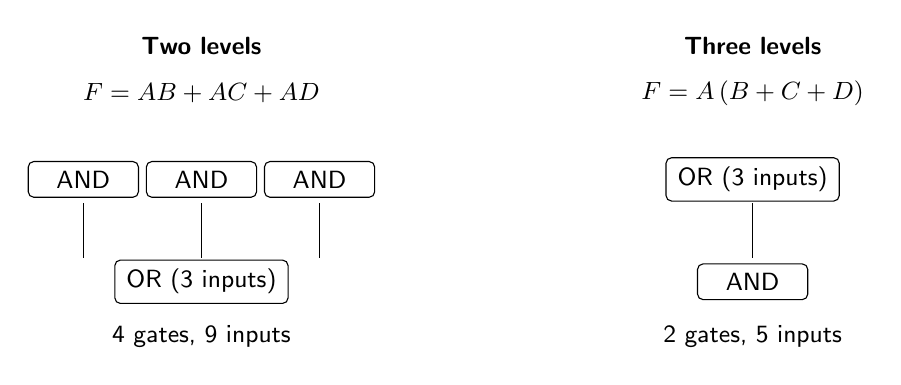
\begin{tikzpicture}[font=\sffamily\small, x=1cm, y=1cm]
  \node at (0,2.2) {\textbf{Two levels}};
  \node at (0,1.6) {$F = AB + AC + AD$};
  \node[draw, rounded corners=2pt, minimum width=14mm] at (-1.5,0.5) {AND};
  \node[draw, rounded corners=2pt, minimum width=14mm] at (0,0.5) {AND};
  \node[draw, rounded corners=2pt, minimum width=14mm] at (1.5,0.5) {AND};
  \node[draw, rounded corners=2pt, minimum width=22mm] at (0,-0.8) {OR (3 inputs)};
  \draw (-1.5,0.2) -- (-1.5,-0.5); \draw (0,0.2) -- (0,-0.5); \draw (1.5,0.2) -- (1.5,-0.5);
  \node at (0,-1.5) {4 gates, 9 inputs};
  \begin{scope}[xshift=7cm]
  \node at (0,2.2) {\textbf{Three levels}};
  \node at (0,1.6) {$F = A\,(B + C + D)$};
  \node[draw, rounded corners=2pt, minimum width=22mm] at (0,0.5) {OR (3 inputs)};
  \node[draw, rounded corners=2pt, minimum width=14mm] at (0,-0.8) {AND};
  \draw (0,0.2) -- (0,-0.5);
  \node at (0,-1.5) {2 gates, 5 inputs};
  \end{scope}
\end{tikzpicture}
\caption{Factoring out a common multiplier reduces the number of gates, but adds another stage of delay}
\end{figure}

Here it is worth remembering the trade-off: the deeper the circuit, the
smaller it is in area, but the slower in delay (in Chapter~\ref{ch:comb} we
saw that the critical path is the sum of the delays of all the levels). So
the designer, and later the program, look for a golden mean depending on the
required speed.

Our guard example shows the same picture: $ABD+ABC+ACD$ is two levels,
4 gates, 12 inputs, while $A\,(BC+BD+CD)$ is three levels, 5 gates, 11
inputs. There is no gain in gates, only in inputs and in readability. There is
no general recipe; each case has to be counted.

\begin{diybox}[Quine and brackets]
\textbf{Task.} \stars{1} For $F=\Sigma m(0,1,2,5,8,9,10)$ repeat the merging
table on paper and make sure you get the same three implicants. \stars{2} For
$F=\Sigma m(0,1,2,5,6,7)$ find all the prime implicants and explain why there
are two different minimal answers. \stars{3} Factor out common multipliers in
$F=ABC+ABD+ACD+BCD$ and compare the number of gates and the number of levels.

\textbf{In Logra.} The \emph{Designer} tab: build both variants for item 3;
the \emph{RTL} tab: compare the resulting circuits.

\textbf{Expected result.} In item 2 there are two minimal covers:
$\overline{A}\,\overline{B}+B\overline{C}+AC$ and
$\overline{A}\,\overline{C}+\overline{B}C+AB$. In item 3 the common
multiplier cannot be factored out completely (the brackets are nested), and
the gain is small.

\textbf{How to check.} The \emph{Waveforms} tab: both circuit variants give
the same table on all 16 combinations.
\end{diybox}

\begin{warnbox}[Common mistakes]
\begin{itemize}
  \item \textbf{Taking the largest group first.} First look for the ones that
        have only one way to be covered and take those groups (the essential
        ones); only then look at what is left.
  \item \textbf{A group that is not a power of two or not a rectangle.} Three
        cells, six cells, an ``L shape'', a diagonal---these are not groups.
  \item \textbf{Forgetting that the map wraps around.} The four corners are one
        group; the left and right columns, and the top and bottom rows, are
        neighbours.
  \item \textbf{Treating don't-care cells as ones in all groups at once.}
        Each $\times$ is chosen independently; moreover, no $\times$ is
        required to be covered.
\end{itemize}
\end{warnbox}

\begin{ideabox}
Minimization is choosing the smallest set of large groups that covers all the
ones. First take the essential groups, then pick up the rest; don't-care
states make groups larger, but are used only if those inputs really are
impossible. The ``minimal'' form is not always the fastest and not always the
most reliable.
\end{ideabox}

\section{Questions and Problems}
\label{sec:tasks-minimize}

The answers are collected in Appendix~\ref{app:answers}.

\begin{taskbox}[Chapter problems]
\begin{enumerate}
  \item \stars{1}~Minimize $F_1=\Sigma m(0,2,8,10)$, $F_2=\Sigma m(1,3,5,7,9,11,13,15)$ and $F_3=\Sigma m(0,1,2,3)$ of four variables $A,B,C,D$.
  \item \stars{2}~The function ``the BCD digit is even'' is given by the minterms $0,2,4,6,8$, and the combinations $10$--$15$ are don't-cares. Find the minimal form.
  \item \stars{2}~Find the prime implicants of the function $F=\Sigma m(0,1,2,5,6,7)$ of three variables by the Quine---McCluskey method and choose a minimal cover.
  \item \stars{1}~Give an example of a function whose Karnaugh map contains a group that wraps around the edge of the map.
  \item \stars{2}~Why does the number of variables of a function matter more for a board than the number of terms in the minimal form?
  \item \stars{1}~Minimize $F=\Sigma m(4,5,6,7,12,13)$ and check how many literals the answer has compared with the canonical SOP.
  \item \stars{2}~Minimize $F=\Sigma m(0,1,2,8,9,10,12,13)$ of four variables. Hint: the groups wrap around the edge.
  \item \stars{2}~\emph{Find the mistake.} A student minimized $F=\Sigma m(1,5,6,7,11,12,13,15)$ and got $F=BD+\overline{A}\,\overline{C}D+\overline{A}BC+ACD+AB\overline{C}$. The answer is correct in value but not minimal. Which term is redundant and why?
  \item \stars{2}~\emph{Find the mistake.} For $F=\Sigma m(0,3,6,9)$ with the don't-care codes $10$--$15$ a student circled the ones in cells $3,6,9$ with a single ``diagonal'' group and wrote one term for it. What is wrong? With which cells can each of the ones $3$, $6$, $9$ actually be combined?
  \item \stars{2}~The function ``the number is divisible by 3'' is defined for BCD digits: ones on $0,3,6,9$, don't-cares $10$--$15$. Find the minimal form.
  \item \stars{3}~\emph{A project with a criterion.} In the Designer, build the function ``the number lies in the range 3\ldots 9'' in two ways: from two comparators (the lesson ``A number in the range 3\ldots 9'') and from the minimal form with don't-care states. Acceptance criterion: both circuits agree on all the values $0$--$9$; the second way uses fewer blocks.
  \item \stars{3}~\emph{A project with a criterion (a stage of the ``Security Panel'' project).} ``2 of 3'' with a guard: write the minimal form of $y=arm\cdot(ab+ac+bc)$ on a Karnaugh map and build both variants (two levels and with a bracket). Acceptance criterion: the tables agree on all 16 rows, and the number of gates is written down.
  \item \stars{3}~For ``at least two of four'' ($a,b,c,d$) find the minimal form on a Karnaugh map and count the gates. Acceptance criterion: the circuit in the Designer agrees with the map on all 16 rows.
  \item \stars{2}~\emph{Verilog.} Write the function ``the digit is divisible by three'' (ones at $0,3,6,9$, codes $10$--$15$ are don't-care) with \code{case} and \code{default: y = 1'bx;}, and compare it with the minimal form on the digits $0$--$9$.
  \item \stars{3}~\emph{A project with a criterion.} Write ``the number lies in the range $3\ldots9$'' in three ways in Verilog: with comparisons, from the minimal form $F=A+B+CD$, and with \code{case}. Acceptance criterion: on the digits $0$--$9$ the three modules agree on the Waveforms tab; for the codes $10$--$15$ it is written down what each of them gives.
\end{enumerate}
\end{taskbox}

\section{What's Next}

We can now simplify a function of four variables, choose the right groups and
use combinations that never occur. But some functions appear so often that
they were given names and are drawn as ready-made ``bricks'':
\emph{a number turns into a one on one of the lines}, and vice versa. Without
them you cannot select one of several sensors or show a digit on a display. In
the next chapter we will meet them and show the number of a security zone on
a display.
